\documentclass[12pt]{article}
\usepackage{amsmath}
\usepackage{amssymb}
\usepackage{graphicx}
\usepackage{natbib}
\usepackage{url}
\usepackage{xcolor}
\usepackage[colorlinks=true,citecolor={blue!65!black},linkcolor={blue!65!black},urlcolor={blue!65!black}]{hyperref}
\usepackage{amsthm}
\usepackage{booktabs}
\usepackage{algorithm}
\usepackage{algpseudocode}
\renewcommand{\algorithmicrequire}{\textbf{Input:}}
\newtheorem{definition}{Definition}
\newtheorem{proposition}{Proposition}

% Margins: 1 inch all around.
\addtolength{\oddsidemargin}{-.5in}%
\addtolength{\evensidemargin}{-.5in}%
\addtolength{\textwidth}{1in}%
\addtolength{\textheight}{1.3in}%
\addtolength{\topmargin}{-.8in}%

\begin{document}

\def\spacingset#1{\renewcommand{\baselinestretch}%
{#1}\small\normalsize} \spacingset{1}

%%%%%%%%%%%%%%%%%%%%%%%%%%%%%%%%%%%%%%%%%%%%%%%%%%%%%%%%%%%%%%%%%%%%%%%%%%%%%%
% Title page

\title{\bf Engineering Enrollment and Wages: Full-Information Estimation of the Ryoo--Rosen Model}
\author{Max Cheong\thanks{
    Thanks go to Professor Thomas J. Sargent for giving me advice on learning dynamic programming, the Kalman filter and maximum likelihood estimation, which is the toolkit of this paper. Data, code, and replication files are available at \url{https://github.com/maxmaxmaxmaxmaxmax373/ryoo-rosen-mle}.}\hspace{.2cm}\\
    Guanghua School of Management, Peking University\\}
\maketitle

\begin{abstract}
Students choose a field of study four years before they enter the labor market, and they are paid over a career, so enrollment depends both on how strongly students respond to wages and on how they form expectations of future wages. We estimate the Ryoo--Rosen model of the market for engineers by full-information maximum likelihood: the competitive equilibrium is solved as a linear-quadratic planning problem, cast in state-space form with measurement error, and taken to U.S. data for 1968--2010 with the Kalman filter. Enrollment is highly sensitive to persistent wage changes: a permanent 1 percent increase in the relative wage eventually raises the share of students entering engineering by about 6 percent. Yet most swings in engineering degrees come from changes in the attractiveness of the field, which follow a damped cycle of about 22 years, rather than from wages. Whether students distinguish temporary from permanent wage changes, as rational expectations imply, the data cannot tell: a cobweb model, in which they expect the current wage to persist, fits about as well and better matches the comovement of wages and future degrees, but only with a nearly flat demand curve. The estimated demand elasticity therefore depends on how students form expectations.
\end{abstract}

\bigskip
\noindent%
{\it Keywords:} Maximum Likelihood Estimation, Rational Expectations, Kalman Filter, Linear-Quadratic Dynamic Programming, Human Capital Investment
\vfill

\newpage
\spacingset{1.45} % DON'T change the spacing!

%%%%%%%%%%%%%%%%%%%%%%%%%%%%%%%%%%%%%%%%%%%%%%%%%%%%%%%%%%%%%%%%%%%%%%%%%%%%%%
\section{Introduction}\label{sec:intro}

The supply of engineers in the United States has fluctuated sharply. Engineering accounted for 4.2 percent of all bachelor's degrees in 1976, 7.8 percent in 1985, and 4.7 percent in 2000.\footnote{Engineering bachelor's degrees divided by all bachelor's degrees, from \citet{nsf13327}, Table 5.} The rise was preceded by a rise in the relative pay of engineers: between 1972 and 1982, the ratio of the median earnings of engineers to that of all college graduates rose from 1.33 to 1.50.\footnote{Author's calculations from IPUMS CPS ASEC microdata \citep{ipumscps}; Section \ref{sec:data} gives the definitions.} Such episodes are not new: talk of a ``shortage'' of engineers was widespread in the 1950s \citep{arrow1959dynamic}, and declining interest in engineering drew attention again around 1990 \citep{ryoo2004engineering}.

These episodes raise four questions, which organize the paper.
\begin{enumerate}\itemsep0pt
\item \textbf{Supply.} How strongly does the choice of engineering respond to the wages engineers earn?
\item \textbf{Demand.} How elastic is the demand for engineers?
\item \textbf{Sources of the cycle.} What drives the booms and busts in engineering degrees: wages, or changes in the attractiveness of the field?
\item \textbf{Expectations.} Do students distinguish temporary from permanent changes in wages, or do they expect the current wage to persist?
\end{enumerate}

Earlier work has addressed each of them. \citet{freeman1971market,freeman1975supply,freeman1976cobweb} explained cycles in the markets for scientists and engineers with a cobweb model, in which students expect the current wage to persist and the supply they create reaches the market several years later. \citet{siow1984occupational} and \citet{zarkin1985occupational} studied occupational choice among lawyers and teachers under rational expectations, and Zarkin compared his model with a cobweb specification. \citet{ryoo2004engineering} developed a dynamic model of the engineering market in which firms' demand falls with the relative wage, students enroll on the basis of the earnings they expect after graduation, and graduates join the stock of engineers four years after they enroll. Estimating the model equation by equation on U.S. data for 1950--1990, they found a demand elasticity between 1.2 and 2.2 and a long-run elasticity of supply with respect to career prospects between 2.5 and 4.5.

Our contribution is to estimate the Ryoo--Rosen model in a full-information framework, using CPS and NSF data for 1968--2010. We show that the competitive equilibrium solves a linear-quadratic planning problem, solve for its law of motion, write it in state-space form together with measurement error, and estimate all parameters jointly by maximum likelihood with the Kalman filter. The framework imposes the restrictions that rational expectations place across the demand, enrollment, and stock equations; it treats expected lifetime earnings, which are not observed, as a function of the model's state rather than measuring them from earnings profiles or instrumenting them; and it accounts for noise in the survey data. Within it we let demand and preference shocks follow unrestricted second-order autoregressions, which allow for cycles, and we construct confidence intervals from the profile likelihood. Because a cobweb model fits into the same likelihood, we can also compare the two forms of expectations directly.

Our answers are as follows. Enrollment is highly sensitive to persistent changes in wages: a permanent 1 percent increase in the relative wage eventually raises the share of students choosing engineering by about 6 percent. The demand elasticity is about 1.6, in line with \citet{ryoo2004engineering}. Yet the large swings in engineering degrees come mainly from changes in the attractiveness of the field, which follow a damped cycle of about 22 years, rather than from wages.

Whether students distinguish temporary from permanent wage changes, the data cannot tell. A cobweb model, in which students expect the current wage to persist, fits about as well as the rational-expectations model and better matches the comovement of wages and future degrees, but only with a nearly flat demand curve. The answer to the fourth question therefore matters for the second: under the cobweb, the demand elasticity is almost four times as large.

The method follows \citet{hansen1980formulating}, who showed how to estimate linear rational-expectations models subject to their cross-equation restrictions, \citet{sargent1989two}, who added measurement error and the Kalman filter, and \citet{hansen2013recursive}. Applications include dynamic labor demand \citep{sargent1978estimation}, time to build \citep{altug1989time}, overtime \citep{hall1996overtime}, and hybrid DSGE--VAR models \citep{ireland2004method}. We apply it to a labor market with a training lag, in which the stock of workers moves slowly and the expected returns to entry are not observed; the cost is that misspecification in any one equation affects all the estimates.

Section \ref{sec:model} presents the model and Section \ref{sec:data} the data. Section \ref{sec:estimation} reports the estimates and the fit of the model, Section \ref{sec:dynamics} studies the dynamics, Section \ref{sec:cobweb} compares rational and cobweb expectations, and Section \ref{sec:conclusion} concludes.

%%%%%%%%%%%%%%%%%%%%%%%%%%%%%%%%%%%%%%%%%%%%%%%%%%%%%%%%%%%%%%%%%%%%%%%%%%%%%%
\section{The Model}\label{sec:model}

We follow \citet{ryoo2004engineering}. Time is discrete, and a period is one year. All variables are log ratios of engineers to all college graduates, measured as deviations from trend: $w_t$ is the relative wage, $N_t$ the relative stock of engineers, and $n_t$ the relative share of students beginning college in year $t$ who choose engineering, which we call the enrollment share. Training takes four years, so the degree share is $\pi_t = n_{t-4}$. A representative firm demands engineering services, and a representative household chooses enrollment and owns the stock of engineers. Both take the wage as given.

Two shocks drive the model. A demand shock $\theta_t$ shifts the marginal product of engineering services, and a preference shock $\psi_t$ shifts the attractiveness of engineering to students. Each follows a stationary second-order autoregression,
\begin{align}
  \theta_{t+1} &= a^{\theta}_{1}\,\theta_t + a^{\theta}_{2}\,\theta_{t-1} + \sigma_{\theta}\,\varepsilon^{\theta}_{t+1}, \label{eq:theta}\\
  \psi_{t+1}   &= a^{\psi}_{1}\,\psi_t + a^{\psi}_{2}\,\psi_{t-1} + \sigma_{\psi}\,\varepsilon^{\psi}_{t+1}, \label{eq:psi}
\end{align}
where $\varepsilon^{\theta}_t$ and $\varepsilon^{\psi}_t$ are independent i.i.d.\ standard normal innovations. We do not restrict the roots to be real. When $a_1^{2}+4a_2<0$, the roots are a complex pair $re^{\pm i\omega}$, and the impulse response, $r^{h}\sin((h+1)\omega)/\sin\omega$, is an oscillation with a period of $2\pi/\omega$ years that decays at rate $r=\sqrt{-a_2}$. The discount factor is fixed at $\beta = 0.96$.

\subsection{Firms, Households, and the Stock of Engineers}\label{sec:agents}

\paragraph{The firm.} The firm chooses its use of engineering services $\{N^{d}_t\}$ to maximize
\begin{equation}\label{eq:firm}
  E_0 \sum_{t=0}^{\infty} \beta^{t}
  \Big[ (f_1 + \theta_t)\, N^{d}_t - \tfrac{f_2}{2} (N^{d}_t)^{2} - w_t N^{d}_t \Big], \qquad f_2>0 .
\end{equation}
The problem is static, and the first-order condition equates the marginal product of engineering services with the wage. The constant $f_1$ affects only the mean wage and drops out in deviations from trend, which gives the inverse demand curve
\begin{equation}\label{eq:demand}
  w_t = -f_2 N^{d}_t + \theta_t .
\end{equation}
Because the variables are in logs, $1/f_2$ is the elasticity of demand.

\paragraph{The stock of engineers.} If a fraction $1-\delta$ of engineers leaves the profession each year and students graduate after four years, the number of engineers evolves as $L_{t+1} = \delta L_t + S_{t-3}$, where $S_t$ is the number of students who begin engineering in year $t$. Log-linearizing around a balanced growth path with growth rate $g$, and subtracting the same equation for all college graduates, gives (Appendix \ref{app:stock})
\begin{equation}\label{eq:stock}
  N_{t+1} = \lambda N_t + (1-\lambda)\, n_{t-3}, \qquad \lambda = \frac{\delta}{1+g} .
\end{equation}
The parameter $\lambda$ is the share of incumbents in next year's stock. Because each graduating cohort is small relative to the stock, the stock adjusts slowly.

\paragraph{The household.} The household chooses the enrollment share $\{n_t\}$ to maximize
\begin{equation}\label{eq:household}
  E_0 \sum_{t=0}^{\infty} \beta^{t}
  \Big[ w_t N^{h}_t - \tfrac{d}{2}\, n_t^{2} + d\,\psi_t\, n_t \Big]
  \quad \text{subject to} \quad
  N^{h}_{t+1} = \lambda N^{h}_t + (1-\lambda)\, n_{t-3} .
\end{equation}
The first term is the wage income of the stock of engineers that the household owns. The marginal cost of enrollment, $d\,n_t$, rises with the enrollment share because potential students differ in ability and in taste for engineering, and the preference shock adds a nonpecuniary return $d\,\psi_t$ per entrant, so the net marginal cost of enrollment is $d\,(n_t - \psi_t)$. A cohort that enrolls in year $t$ raises the stock in year $t+4+j$ by $(1-\lambda)\lambda^{j}$, and the first-order condition for $n_t$ is (Appendix \ref{app:household})
\begin{equation}\label{eq:hhfocmain}
  d\,(n_t - \psi_t) = (1-\lambda)\, E_t \sum_{j=0}^{\infty} \beta^{4+j} \lambda^{j}\, w_{t+4+j} .
\end{equation}
Rearranging gives the enrollment equation
\begin{equation}\label{eq:enrollment}
  n_t = \frac{1-\lambda}{d}\, V_t + \psi_t , \qquad
  V_t = \beta^{4}\, E_t \sum_{j=0}^{\infty} (\beta\lambda)^{j}\, w_{t+4+j} .
\end{equation}
$V_t$ is the career value of engineering: the expected present value of the relative wages a cohort earns after graduation, weighted by its declining share in the stock. A unit increase in $V_t$ raises enrollment by $(1-\lambda)/d$. A permanent 1 percent increase in the relative wage raises $V_t$ by $\beta^{4}/(1-\beta\lambda)$, so the long-run entry elasticity is
\begin{equation}\label{eq:lrelasticity}
  \eta^{LR} = \frac{(1-\lambda)\,\beta^{4}}{d\,(1-\beta\lambda)} .
\end{equation}

\paragraph{Expectations.} In the baseline, expectations are rational: $E_t$ is the mathematical expectation conditional on the state in year $t$. Students then forecast how their peers' choices will affect future wages. Section \ref{sec:cobweb} considers cobweb expectations instead, under which students expect the current wage to persist, $E_t w_{t+j} = w_t$. Then $V_t = \beta^{4} w_t/(1-\beta\lambda)$, and
\begin{equation}\label{eq:cobweb}
  n_t = \eta\, w_t + \psi_t, \qquad \eta = \frac{(1-\lambda)\,\beta^{4}}{d\,(1-\beta\lambda)} .
\end{equation}
Enrollment then moves only with the current wage, and students no longer anticipate that their peers' entry will depress future wages. Under the cobweb we estimate $\eta$ in place of $d$.

\subsection{Equilibrium and Solution}\label{sec:planner}

\begin{definition}
A rational expectations competitive equilibrium is a collection of stochastic processes $\{w_t, N^{d}_t, N^{h}_t, n_t\}$ with bounded second moments such that (i) given $\{w_t\}$, $\{N^{d}_t\}$ solves the firm's problem \eqref{eq:firm}; (ii) given $\{w_t\}$, $\{n_t, N^{h}_t\}$ solves the household's problem \eqref{eq:household}; and (iii) the market clears, $N^{d}_t = N^{h}_t \equiv N_t$.
\end{definition}

\noindent Enrollment depends on expected wages, which in turn depend on enrollment. The following result removes this fixed-point problem. Consider the planning problem
\begin{equation}\label{eq:planner}
  \max_{\{n_t\}} \; E_0 \sum_{t=0}^{\infty} \beta^{t}
  \Big[ \theta_t N_t - \tfrac{f_2}{2} N_t^{2} - \tfrac{d}{2} n_t^{2} + d\,\psi_t\, n_t \Big]
  \quad \text{subject to}\quad \eqref{eq:theta}\text{--}\eqref{eq:stock} ,
\end{equation}
whose objective is the sum of the firm's and the household's objectives once the wage bill and wage income cancel.

\begin{proposition}\label{prop:equivalence}
An allocation $\{N_t, n_t\}$ is a competitive equilibrium allocation if and only if it solves \eqref{eq:planner}, with equilibrium wage $w_t = \theta_t - f_2 N_t$. The equilibrium is unique.
\end{proposition}

\noindent The proof, in Appendix \ref{app:equivalence}, shows that the planner's first-order condition coincides with the household's once the firm's condition \eqref{eq:demand} is substituted for the wage.

\paragraph{Matrix form.} Let the state and the control be
\[
  X_t = \big(N_t,\; n_{t-1},\; n_{t-2},\; n_{t-3},\; n_{t-4},\; \theta_t,\; \psi_t,\; \theta_{t-1},\; \psi_{t-1}\big)', \qquad u_t = n_t .
\]
The constraints and the period return in \eqref{eq:planner} take the form
\begin{equation}\label{eq:transition}
  X_{t+1} = A X_t + B u_t + C \varepsilon_{t+1}, \qquad
  r(X_t, u_t) = X_t' R X_t + Q u_t^{2} + 2 u_t W X_t ,
\end{equation}
with $\varepsilon_t = (\varepsilon^{\theta}_t, \varepsilon^{\psi}_t)'$ and the matrices given in Appendix \ref{app:lq}.

\paragraph{Solution.} The value function is quadratic, $v(X) = X'PX + c$, and satisfies the Bellman equation
\begin{equation}\label{eq:bellman}
  X'PX + c = \max_{u} \big\{ X'RX + Qu^{2} + 2uWX + \beta\,(AX+Bu)'P(AX+Bu) + \beta\,\mathrm{tr}(C'PC) + \beta c \big\} .
\end{equation}
The first-order condition gives the decision rule
\begin{equation}\label{eq:F}
  u_t = -F X_t, \qquad F = (Q + \beta B'PB)^{-1}(W + \beta B'PA) ,
\end{equation}
and matching the quadratic terms shows that $P$ solves the algebraic Riccati equation
\begin{equation}\label{eq:riccati}
  P = R + \beta A'PA - (W' + \beta A'PB)(Q + \beta B'PB)^{-1}(W + \beta B'PA) .
\end{equation}
The second-order condition holds: the block of $P$ for the endogenous states is negative semidefinite because the objective is concave in them, and $B$ selects only $n_{t-1}$, so $Q + \beta B'PB \le -d/2 < 0$. Because $F$ does not depend on $C$, certainty equivalence holds. We solve \eqref{eq:riccati} with a standard solver after rescaling $(A, B)$ by $\sqrt{\beta}$. Substituting \eqref{eq:F} into \eqref{eq:transition} gives the equilibrium law of motion
\begin{equation}\label{eq:lawofmotion}
  X_{t+1} = M X_t + C \varepsilon_{t+1}, \qquad M = A - BF .
\end{equation}

\paragraph{Career value.} Let $G_w$ be the row vector with $w_t = G_w X_t$. Since $E_t X_{t+k} = M^{k} X_t$, the career value in \eqref{eq:enrollment} is
\begin{equation}\label{eq:Vclosed}
  V_t = \beta^{4} \sum_{j=0}^{\infty} (\beta\lambda)^{j}\, G_w M^{4+j} X_t
      = \beta^{4}\, G_w M^{4} \big(I - \beta\lambda M\big)^{-1} X_t .
\end{equation}
Although $V_t$ forecasts wages four or more years ahead, it is linear in the current state, so any shock moves $V_t$ and enrollment at once. Under cobweb expectations no planning problem is needed: by \eqref{eq:demand} and \eqref{eq:cobweb}, $n_t = -\eta f_2 N_t + \eta\,\theta_t + \psi_t \equiv K X_t$, and $X_{t+1} = (A+BK) X_t + C\varepsilon_{t+1}$. Under either form of expectations, $w_t$, $N_t$, and $\pi_t$ are linear functions of $X_t$.

%%%%%%%%%%%%%%%%%%%%%%%%%%%%%%%%%%%%%%%%%%%%%%%%%%%%%%%%%%%%%%%%%%%%%%%%%%%%%%
\section{Data}\label{sec:data}

We use annual U.S. data for 1968--2010, 43 observations in all. The relative wage and the relative stock come from CPS ASEC microdata harmonized by IPUMS \citep{ipumscps}. Engineers are employed workers in OCC1990 codes 044--059, and college graduates are persons with four or more years of college (EDUC $\geq 110$). For each year we compute the median annual earnings of the two groups, $W^{E}_t$ and $W^{C}_t$, and their weighted counts, $L^{E}_t$ and $L^{C}_t$.\footnote{Years are survey years; the CPS ASEC asks about earnings in the previous calendar year.} The degree share uses the numbers of engineering and of all bachelor's degrees, $D^{E}_t$ and $D^{A}_t$, from \citet{nsf13327}, Table 5. The NSF did not publish degrees by field for 1999, and we interpolate that year linearly. The observed series are
\begin{equation}\label{eq:datadef}
  \hat w_t = \log \frac{W^{E}_t}{W^{C}_t}, \qquad
  \hat N_t = \log \frac{L^{E}_t}{L^{C}_t}, \qquad
  \hat \pi_t = \log \frac{D^{E}_t}{D^{A}_t} .
\end{equation}
Taking ratios removes factors common to both groups, such as inflation and the growth of the college-educated population. The three series have different trends: the relative stock falls by about 2.6 log points a year and the degree share by about 0.5, while the relative wage has almost none. We therefore remove a separate linear trend from each series,
\begin{equation}\label{eq:detrend}
  x_t = a_x + b_x\, t + \tilde x_t, \qquad x \in \{\hat w, \hat N, \hat \pi\},
\end{equation}
and use the residuals $\tilde w_t$, $\tilde N_t$, and $\tilde\pi_t$ as observations. Figure \ref{fig:series} plots the series. After detrending, the degree share fluctuates the most: it lies 33 log points below trend in 1976 and 35 log points above trend in 1985.

\begin{figure}[!htb]
\centering
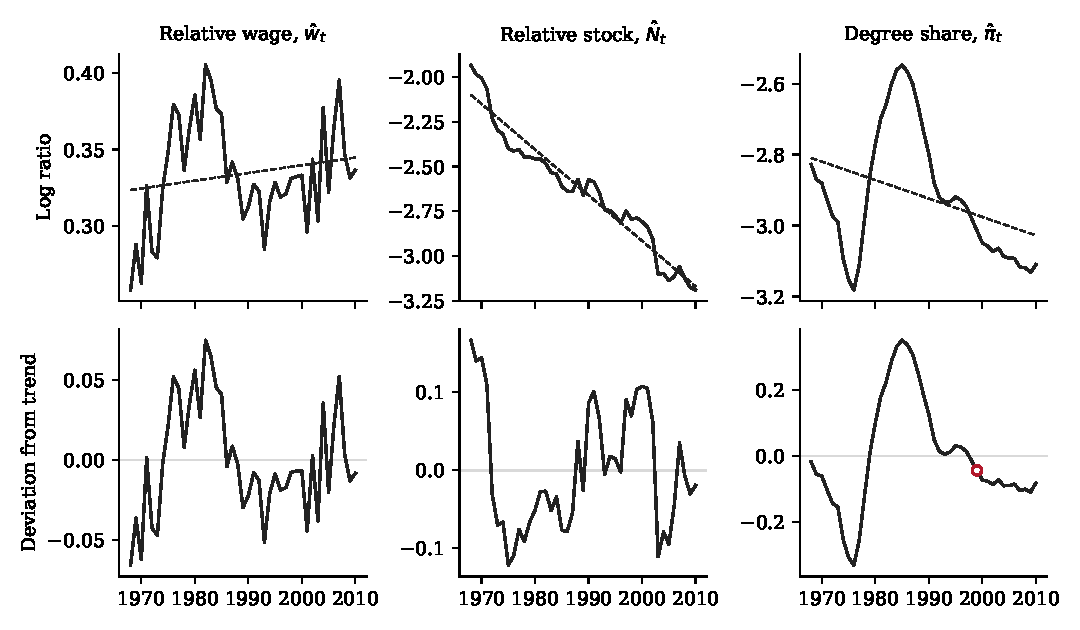
\includegraphics[width=0.72\linewidth]{fig_data_series.pdf}
\caption{Relative wage, relative stock, and degree share, 1968--2010}\label{fig:series}
\begin{minipage}{0.85\linewidth}\footnotesize
\textit{Notes:} Top: the log ratios in \eqref{eq:datadef} (solid) and their linear trends (dashed). Bottom: the detrended series. The open circle marks the interpolated value for 1999. \textit{Sources:} CPS ASEC (IPUMS); NSF 13-327, Table 5.
\end{minipage}
\end{figure}

%%%%%%%%%%%%%%%%%%%%%%%%%%%%%%%%%%%%%%%%%%%%%%%%%%%%%%%%%%%%%%%%%%%%%%%%%%%%%%
\section{Estimation}\label{sec:estimation}

\subsection{The Likelihood Function}\label{sec:likelihood}

\paragraph{Observation equation.} Let $y_t = (\tilde w_t, \tilde N_t, \tilde \pi_t)'$. Each observation equals its model counterpart, $G X_t$, plus a measurement error:
\begin{equation}\label{eq:obs}
  y_t = G X_t + v_t, \qquad
  v^{x}_{t+1} = D_x\, v^{x}_t + \sigma_x\, e^{x}_{t+1}, \quad x \in \{w, N, \pi\},
\end{equation}
where the $e^{x}_t$ are standard normal and independent of each other and of the structural shocks. Measurement error in the CPS series is not negligible. The survey contains only 611 to 1,409 engineers a year, and the measured stock falls by 17.7 log points in 2003, when the CPS adopted a new occupational classification \citep{bls_cpsoccind}, although new graduates add only about 4 percent to the stock each year. Because about half of the CPS sample overlaps between adjacent years, we allow these errors to be serially correlated. The degree share comes from administrative records, and we set $D_\pi = 0$.

\paragraph{Likelihood.} Adding the measurement errors to the state, $s_t = (X_t', v_t')'$, the law of motion \eqref{eq:lawofmotion} and the observation equation \eqref{eq:obs} form the state-space system
\begin{equation}\label{eq:ssm}
  s_{t+1} = \mathcal{M} s_t + \mathcal{C} \epsilon_{t+1}, \qquad y_t = \mathcal{G} s_t ,
\end{equation}
where $\epsilon_t$ collects the two structural shocks and the three measurement innovations (Appendix \ref{app:ssm}). Let $\hat{s}_t = E[s_t \mid y^{t-1}]$ with $y^{t-1} = (y_1, \dots, y_{t-1})$. The Kalman filter gives the innovations representation
\begin{equation}\label{eq:innovrep}
  \hat{s}_{t+1} = \mathcal{M}\hat{s}_t + K_t a_t, \qquad y_t = \mathcal{G}\hat{s}_t + a_t , \qquad a_t \mid y^{t-1} \sim N(0, \Omega_t),
\end{equation}
where the innovation $a_t$ is the part of $y_t$ that cannot be predicted from past observations, and the gain $K_t$ and covariance $\Omega_t$ follow from the filtering recursions started at the stationary distribution (Appendix \ref{app:recursion}). The innovations are serially independent and in one-to-one correspondence with the observations, so the joint density of the sample is the product of the innovation densities (Appendix \ref{app:ped}):
\begin{equation}\label{eq:loglik}
  \log L = \sum_{t=1}^{T} \Big[ -\tfrac{3}{2}\log 2\pi - \tfrac12 \log \det \Omega_t - \tfrac12\, a_t' \Omega_t^{-1} a_t \Big] .
\end{equation}

\paragraph{Estimation.} The parameter vector is
\begin{equation}\label{eq:paramvec}
  \Theta = \big(f_2,\, d,\, \lambda,\; a^{\theta}_1,\, a^{\theta}_2,\, \sigma_\theta,\; a^{\psi}_1,\, a^{\psi}_2,\, \sigma_\psi,\; \sigma_w,\, D_w,\, \sigma_N,\, D_N,\, \sigma_\pi\big)' \in \mathcal{P} \subset \mathbb{R}^{14},
\end{equation}
where $\mathcal{P}$ requires $f_2$, $d$, and the standard deviations to be positive, $\lambda \in (0,1)$, $|D_w|, |D_N| < 1$, and both autoregressions to be stationary. The estimator is $\hat\Theta = \arg\max_{\Theta \in \mathcal{P}} \log L(\Theta)$. Evaluating $\log L(\Theta)$ takes three steps, listed in Algorithm \ref{alg:loglik}: solve the planning problem for $M$, build the state-space system \eqref{eq:ssm}, and run the Kalman filter. If the Riccati equation has no solution, $\mathcal{M}$ is not stable, or some $\Omega_t$ is not positive definite, we set $\log L = -10^{10}$.

\begin{algorithm}[!htb]
\caption{Evaluating the log likelihood $\log L(\Theta)$}\label{alg:loglik}
\begin{algorithmic}[1]
\Require parameters $\Theta$; observations $y_1, \dots, y_T$
\State Construct $A, B, C, R, Q, W$ from $\Theta$; solve \eqref{eq:riccati} for $P$; set $F$ by \eqref{eq:F} and $M = A - BF$
\State Construct $\mathcal{M}, \mathcal{C}, \mathcal{G}$; set $\hat{s}_1 = 0$, $\Sigma_1 = \mathcal{M}\Sigma_1\mathcal{M}' + \mathcal{C}\mathcal{C}'$, and $\log L \gets 0$
\For{$t = 1, \dots, T$}
  \State $a_t \gets y_t - \mathcal{G}\hat{s}_t$, \quad $\Omega_t \gets \mathcal{G}\Sigma_t\mathcal{G}'$, \quad $\log L \gets \log L - \tfrac{3}{2}\log 2\pi - \tfrac12 \log\det\Omega_t - \tfrac12\, a_t'\Omega_t^{-1}a_t$
  \State $K_t \gets \mathcal{M}\Sigma_t\mathcal{G}'\Omega_t^{-1}$, \quad $\hat{s}_{t+1} \gets \mathcal{M}\hat{s}_t + K_t a_t$, \quad $\Sigma_{t+1} \gets (\mathcal{M} - K_t\mathcal{G})\Sigma_t(\mathcal{M} - K_t\mathcal{G})' + \mathcal{C}\mathcal{C}'$
\EndFor
\State \Return $\log L$
\end{algorithmic}
\end{algorithm}

\paragraph{Optimization and inference.} We impose $\mathcal{P}$ by reparametrization: $f_2$, $d$, and the standard deviations are exponentials of unconstrained parameters, $\lambda$ is a logistic function, $a_2$, $D_w$, and $D_N$ are hyperbolic tangents, and $a_1 = (1 - a_2)\tanh(z)$, which keeps each autoregression stationary. We maximize with the Nelder--Mead method, then BFGS, then Nelder--Mead again from the BFGS solution. From eight starting values, seven reach the same estimate; the eighth stops at a lower local maximum ($\log L = 259.45$). Standard errors come from the inverse of the numerical Hessian; $\sigma_\pi$, estimated on the boundary of $\mathcal{P}$, is held fixed. Because the likelihood can be asymmetric, we also report profile likelihood intervals: fixing one parameter at $x$ and re-maximizing over the other 13 gives $\log L_p(x)$, and the values of $x$ with
\begin{equation}\label{eq:profile}
  LR(x) = 2\,\big[\log L(\hat\Theta) - \log L_p(x)\big] \le 3.84
\end{equation}
form a 95 percent confidence interval.

\subsection{Estimates}\label{sec:estimates}

Table \ref{tab:estimates} reports the estimates, which answer the first two questions, and Figure \ref{fig:profile} plots $LR(x)$ for nine parameters.

\begin{table}[!htb]
\centering
\caption{Parameter estimates}\label{tab:estimates}
\small
\renewcommand{\arraystretch}{0.9}
\begin{tabular}{@{}llcccc@{}}
\toprule
 & & & & \multicolumn{2}{c}{Profile 95\% interval} \\
\cmidrule(l){5-6}
Parameter & Description & Estimate & S.E. & Lower & Upper \\
\midrule
\multicolumn{6}{@{}l}{\textit{A. Demand, enrollment, and stock}} \\
$f_2$ & Slope of inverse demand & 0.638 & (0.487) & 0.135 & $>6.32$ \\
$d$ & Enrollment cost slope & 0.075 & (0.054) & $<0.009$ & 0.439 \\
$\lambda$ & Share of incumbents in the stock & 0.955 & (0.029) & 0.895 & $>0.995$ \\[2pt]
\multicolumn{6}{@{}l}{\textit{B. Demand shock $\theta$}} \\
$a^{\theta}_1$ & AR(2) coefficient & 0.697 & (0.319) & $-0.090$ & $>1.656$ \\
$a^{\theta}_2$ & AR(2) coefficient & 0.176 & (0.324) & $<-0.797$ & 0.646 \\
$\sigma_\theta$ & Innovation s.d. & 0.0137 & (0.0049) & $<0.005$ & 0.030 \\[2pt]
\multicolumn{6}{@{}l}{\textit{C. Preference shock $\psi$}} \\
$a^{\psi}_1$ & AR(2) coefficient & 1.735 & (0.086) & 1.541 & 1.876 \\
$a^{\psi}_2$ & AR(2) coefficient & $-0.815$ & (0.086) & $-0.954$ & $-0.618$ \\
$\sigma_\psi$ & Innovation s.d. & 0.0329 & (0.0072) & 0.022 & 0.053 \\[2pt]
\multicolumn{6}{@{}l}{\textit{D. Measurement error}} \\
$\sigma_w$ & Wage: innovation s.d. & 0.0180 & (0.0038) & $<0.010$ & 0.026 \\
$D_w$ & Wage: persistence & $-0.098$ & (0.267) & $<-0.900$ & $>0.704$ \\
$\sigma_N$ & Stock: innovation s.d. & 0.0492 & (0.0053) & 0.040 & 0.062 \\
$D_N$ & Stock: persistence & 0.729 & (0.108) & 0.507 & 0.931 \\
$\sigma_\pi$ & Degree share: s.d. & 0 & --- & 0 & 0.009 \\[2pt]
\multicolumn{6}{@{}l}{\textit{E. Implied quantities}} \\
$1/f_2$ & Demand elasticity & 1.57 & (1.20) & & \\
$(1-\lambda)/d$ & Coefficient on $V_t$ & 0.59 & (0.38) & & \\
$\eta^{LR}$ & Long-run entry elasticity & 6.07 & (3.63) & & \\
 & Preference shock: modulus, period & 0.90, 22.3 yr & & & \\
\midrule
$\log L$ & Maximized log likelihood & 260.47 & & & \\
\bottomrule
\end{tabular}
\par\medskip
\begin{minipage}{0.95\linewidth}\footnotesize
\textit{Notes:} $T=43$; $\beta = 0.96$ is fixed. Standard errors are from the inverse numerical Hessian, with $\sigma_\pi$ held at its boundary value; those of implied quantities use the delta method. Profile intervals contain the values with $LR(x) \le 3.84$; ``$>$'' and ``$<$'' mean that the bound is not reached within the grid.
\end{minipage}
\end{table}

\paragraph{Demand.} The estimate of $f_2$ is 0.64, so the demand elasticity is $1/f_2 = 1.57$, within the range of 1.2 to 2.2 found by \citet{ryoo2004engineering}. The profile likelihood bounds $f_2$ only from below, at 0.135: the data rule out a nearly flat demand curve, with an elasticity above about 7.4, but not a steep one. An interval of two standard errors would be misleading here, since it includes negative values of $f_2$ that the profile likelihood rejects.

\paragraph{Supply.} The coefficient on $V_t$, $(1-\lambda)/d$, is 0.59: a one-percentage-point increase in career value raises the enrollment share by 0.59 percent. A permanent 1 percent wage increase raises $V_t$ by $\beta^{4}/(1-\beta\lambda) = 10.26$ points, so the long-run entry elasticity is $0.59 \times 10.26 = 6.07$, above the range of 2.5 to 4.5 that \citet{ryoo2004engineering} report for the long-run supply elasticity with respect to career prospects, though imprecisely estimated. The enrollment cost $d$ is bounded only from above, at 0.44: the data rule out enrollment that is insensitive to wages, but not enrollment that is highly sensitive.

\paragraph{Stock.} The estimate of $\lambda$ is 0.955. Since $1-\lambda$ is the share of new graduates in the stock, the average ratio of engineering degrees to engineers over 1968--2010, 0.041, gives an accounting benchmark of $\lambda = 0.959$. The estimate, which uses only the dynamics of the three series, is almost identical.

\paragraph{Shocks.} The demand shock has real roots, 0.89 and $-0.20$, and its parameters are poorly determined. The preference shock is precisely estimated, with profile intervals closed on both sides. Its roots are a complex pair, $0.867 \pm 0.251i$, with modulus 0.90: a damped oscillation with a period of about 22 years. Restricting both shocks to real roots lowers the log likelihood to 258.11. The likelihood ratio statistic, 4.72, exceeds the 5 percent critical value of 3.84, so the restriction is rejected.\footnote{Because the null hypothesis is an inequality, $(a^{\psi}_1)^2 + 4a^{\psi}_2 \ge 0$, its least favorable point lies on the boundary of the real-root region, where the statistic follows an equal mixture of $\chi^2_0$ and $\chi^2_1$ with a 5 percent critical value of 2.71. The conclusion is unchanged.}

\paragraph{Measurement error.} The stock error has a standard deviation of 0.049 and persistence 0.73, against a standard deviation of 0.079 for the detrended stock itself: the stock series is noisy. The wage error has a standard deviation of 0.018, and the data cannot tell whether it is serially correlated. The degree-share error is estimated at zero, on the boundary of the parameter space.\footnote{A zero estimate of a measurement-error variance is known in factor analysis as a Heywood case.}

\begin{figure}[!htb]
\centering
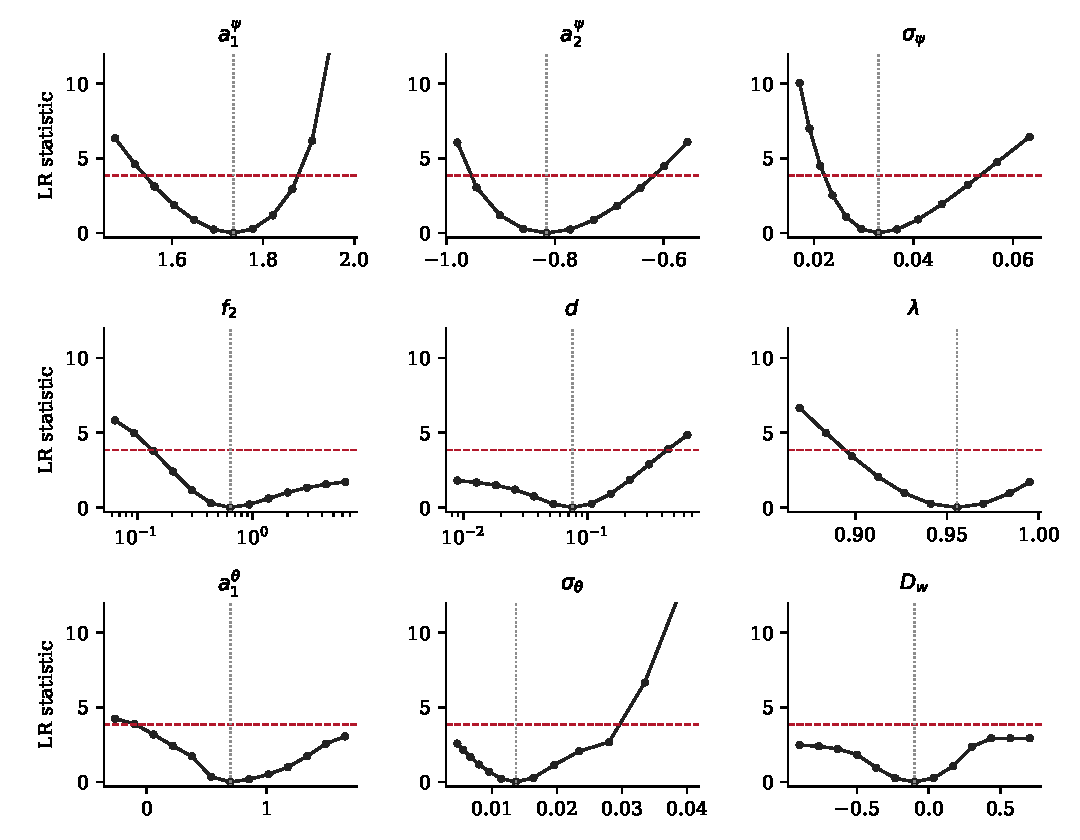
\includegraphics[width=0.66\linewidth]{fig_profile.pdf}
\caption{Profile likelihood for selected parameters}\label{fig:profile}
\begin{minipage}{0.8\linewidth}\footnotesize
\textit{Notes:} Each panel plots $LR(x)$ in \eqref{eq:profile}. Rows: parameters bounded on both sides; bounded on one side; poorly determined. The dashed line is the 5 percent critical value, 3.84; the dotted line marks the estimate. The axes for $f_2$ and $d$ are logarithmic.
\end{minipage}
\end{figure}

\subsection{Model Fit}\label{sec:fit}

The parameters maximize the likelihood rather than match particular moments. To check the fit, we simulate 1,000 samples of 43 years from the estimated model, including measurement error, detrend each as in \eqref{eq:detrend}, and compare the statistics in the data with their distribution across samples (Table \ref{tab:fit}).

\begin{table}[!htb]
\centering
\caption{Data and model moments}\label{tab:fit}
\small
\renewcommand{\arraystretch}{0.9}
\begin{tabular}{@{}lccccc@{}}
\toprule
 & & \multicolumn{4}{c}{Model} \\
\cmidrule(l){3-6}
 & Data & Population & Median & 5\% & 95\% \\
\midrule
\multicolumn{6}{@{}l}{\textit{Standard deviation}} \\
\quad $\tilde w_t$ & 0.035 & 0.037 & 0.028 & 0.021 & 0.040 \\
\quad $\tilde N_t$ & 0.079 & 0.080 & 0.064 & 0.046 & 0.088 \\
\quad $\tilde \pi_t$ & 0.169 & 0.140 & 0.118 & 0.065 & 0.195 \\[2pt]
\multicolumn{6}{@{}l}{\textit{First-order autocorrelation}} \\
\quad $\tilde w_t$ & 0.569 & 0.653 & 0.431 & 0.016 & 0.725 \\
\quad $\tilde N_t$ & 0.765 & 0.778 & 0.657 & 0.408 & 0.816 \\
\quad $\tilde \pi_t$ & 0.957 & 0.947 & 0.934 & 0.869 & 0.962 \\[2pt]
\multicolumn{6}{@{}l}{\textit{Correlation of the wage with the future degree share}} \\
\quad $\mathrm{corr}(\tilde w_t, \tilde \pi_{t+4})$ & 0.750 & 0.286 & 0.352 & $-0.118$ & 0.691 \\
\quad $\mathrm{corr}(\tilde w_t, \tilde \pi_{t+5})$ & 0.763 & 0.319 & 0.365 & $-0.072$ & 0.711 \\
\bottomrule
\end{tabular}
\par\medskip
\begin{minipage}{0.85\linewidth}\footnotesize
\textit{Notes:} Population moments are from the stationary distribution of the model (Appendix \ref{app:moments}). The median and percentiles are across 1,000 simulated 43-year samples, each including measurement error and detrended as in \eqref{eq:detrend}.
\end{minipage}
\end{table}

The model reproduces the volatility and persistence of all three series: each standard deviation and first-order autocorrelation in the data lies within the 5th--95th percentile range of the simulated samples. What the model has difficulty matching is the correlation between the wage and the future degree share. In the data, $\mathrm{corr}(\tilde w_t, \tilde \pi_{t+4}) = 0.75$: years with high wages see more students enroll and, four years later, more graduates. The model reproduces the shape of the correlation function (Figure \ref{fig:cwcorr}), but for leads of three to six years the data lie above the 95th percentile of the simulated samples. Section \ref{sec:irf} shows that this gap follows from rational expectations.

%%%%%%%%%%%%%%%%%%%%%%%%%%%%%%%%%%%%%%%%%%%%%%%%%%%%%%%%%%%%%%%%%%%%%%%%%%%%%%
\section{Dynamics}\label{sec:dynamics}

This section turns to the third question: how shocks propagate and where the fluctuations come from.

\subsection{Impulse Responses}\label{sec:irf}

In year 0 the economy is hit by a one-standard-deviation demand or preference shock, and no further shocks occur. By \eqref{eq:lawofmotion}, the state $h$ years after shock $j$ is $X_h = M^{h}Ce_j$, where $e_j$ is the $j$th unit vector, and the wage and enrollment are $w_h = G_wX_h$ and $n_h = -FX_h$. Figure \ref{fig:irf} plots the responses.

\begin{figure}[!htb]
\centering
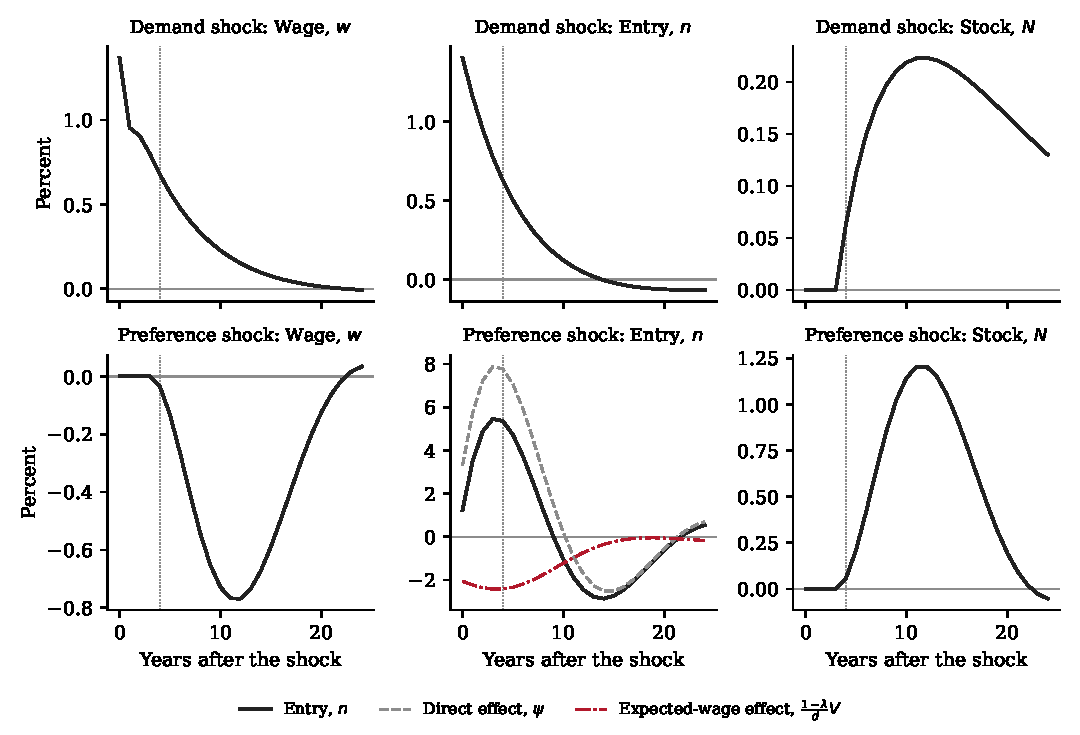
\includegraphics[width=0.7\linewidth]{fig_irf.pdf}
\caption{Responses to one-standard-deviation demand and preference shocks}\label{fig:irf}
\begin{minipage}{0.85\linewidth}\footnotesize
\textit{Notes:} Top row: demand shock; bottom row: preference shock. Columns: percentage deviations of the relative wage, the enrollment share, and the relative stock. The middle bottom panel splits enrollment into the direct effect of preferences, $\psi_h$ (dashed), and the effect of expected wages, $\frac{1-\lambda}{d}V_h$ (dash-dotted). The vertical dotted line marks year 4, when the year-0 cohort graduates.
\end{minipage}
\end{figure}

There are two main points to take away from Figure \ref{fig:irf}. First, under rational expectations students look ahead and do not chase temporarily high wages. A demand shock raises the relative wage by 1.37 percent on impact, and enrollment rises by 1.40 percent in the same year, long before the higher wage reaches graduates. The wage increase, however, decays by half in about four years. Students anticipate this, so the career value $V_t$ rises by only 2.4 percentage points, compared with 14.0 points if the same wage increase were permanent, and enrollment responds only about one-sixth as much. This is why the model understates the correlation between the wage and the future degree share: wage fluctuations induce only small changes in enrollment, so the degree share moves mainly with preferences that are unrelated to wages.

Second, the preference shock is largely self-offsetting. The shock is 3.29 percent on impact, but enrollment rises by only 1.24 percent, about 37 percent of the shock. Students foresee that they and the cohorts that follow will enter the field together, so that four years later the stock will rise and the wage will fall. The career value therefore falls at once and offsets about 63 percent of the direct effect. The preference shock itself oscillates with a period of about 22 years; the stock peaks at 1.20 percent in years 11--12, when the wage reaches its trough of $-0.77$ percent. Under both shocks the stock adjusts slowly: without new entry, a deviation of the stock from steady state has a half-life of 15.2 years, so the effects of a single shock last for more than a decade.

\subsection{Variance Decomposition}\label{sec:vardecomp}

The five shocks are independent, so the variance of each series can be split by shock (Appendix \ref{app:moments}). Table \ref{tab:vardecomp} reports the result.

\begin{table}[!htb]
\centering
\caption{Variance decomposition}\label{tab:vardecomp}
\small
\renewcommand{\arraystretch}{0.9}
\begin{tabular}{@{}lccc@{\hspace{2.5em}}ccc@{}}
\toprule
 & \multicolumn{3}{c}{Observed series} & \multicolumn{3}{c}{Model variables} \\
\cmidrule(r{2.5em}){2-4}\cmidrule(l){5-7}
 & $\tilde w_t$ & $\tilde N_t$ & $\tilde\pi_t$ & $w_t$ & $N_t$ & $n_t$ \\
\midrule
Demand shock & 0.42 & 0.01 & 0.03 & 0.56 & 0.07 & 0.03 \\
Preference shock & 0.34 & 0.18 & 0.97 & 0.44 & 0.93 & 0.97 \\
Measurement error & 0.24 & 0.81 & 0.00 & & & \\
\bottomrule
\end{tabular}
\par\medskip
\begin{minipage}{0.85\linewidth}\footnotesize
\textit{Notes:} Shares of the stationary variance contributed by each shock; each column sums to one. Measurement error is the series' own. The model variables exclude measurement error.
\end{minipage}
\end{table}

Three results stand out. First, about 97 percent of the variance of enrollment and of the degree share comes from the preference shock. Consistent with Section \ref{sec:irf}, the large swings in the choice of major come mainly from changes in the attractiveness of engineering, not from wages. Second, 81 percent of the variance of the observed stock comes from measurement error. Third, both shocks matter for wages: the demand shock accounts for 56 percent of the variance of the true wage and the preference shock for 44 percent.

%%%%%%%%%%%%%%%%%%%%%%%%%%%%%%%%%%%%%%%%%%%%%%%%%%%%%%%%%%%%%%%%%%%%%%%%%%%%%%
\section{Rational Expectations versus the Cobweb}\label{sec:cobweb}

This section turns to the fourth question and reports estimates under cobweb expectations \eqref{eq:cobweb}, with the same data and likelihood. The cobweb model replaces $d$ with $\eta$ and also has 14 free parameters.\footnote{The cobweb likelihood has several local maxima. Of six starting values, two reach a solution with $\log L = 259.59$ and $\eta = 0.41$; two reach $\log L = 263.07$, at which $\sigma_\psi \to 0$ and the roots of the preference shock reach the unit circle, so that the shock becomes a deterministic sine wave and the model has no stationary distribution; and two reach $\log L = 261.92$ and $262.00$ with $\eta \approx 5.1$. We exclude the degenerate solution and report the highest maximum among solutions whose roots all have modulus below 0.99.}

\begin{table}[!htb]
\centering
\caption{Rational-expectations and cobweb estimates}\label{tab:cobweb}
\small
\renewcommand{\arraystretch}{0.9}
\begin{tabular}{@{}lcccc@{}}
\toprule
 & \multicolumn{2}{c}{Rational expectations} & \multicolumn{2}{c}{Cobweb} \\
\cmidrule(lr){2-3}\cmidrule(l){4-5}
 & Estimate & S.E. & Estimate & S.E. \\
\midrule
$\log L$ & 260.47 & & 262.00 & \\[2pt]
$f_2$ & 0.638 & (0.487) & 0.167 & (0.246) \\
$d$ & 0.075 & (0.054) & & \\
$\eta$ & & & 5.10 & (1.32) \\
$\lambda$ & 0.955 & (0.029) & 0.946 & (0.031) \\[2pt]
$a^{\theta}_1$ & 0.697 & (0.319) & 1.877 & (0.084) \\
$a^{\theta}_2$ & 0.176 & (0.324) & $-0.936$ & (0.081) \\
$\sigma_\theta$ & 0.0137 & (0.0049) & 0.0019 & (0.0010) \\
$a^{\psi}_1$ & 1.735 & (0.086) & 1.587 & (0.142) \\
$a^{\psi}_2$ & $-0.815$ & (0.086) & $-0.732$ & (0.144) \\
$\sigma_\psi$ & 0.0329 & (0.0072) & 0.0217 & (0.0046) \\[2pt]
$\sigma_w$, $D_w$ & 0.0180, $-0.098$ & & 0.0214, $-0.052$ & \\
$\sigma_N$, $D_N$ & 0.0492, 0.729 & & 0.0491, 0.729 & \\
$\sigma_\pi$ & 0 & & 0.0037 & \\
\midrule
Demand elasticity $1/f_2$ & 1.57 & & 5.99 & \\
Entry elasticity & 6.07 & & 5.10 & \\
Demand shock: modulus, period & 0.89, --- & & 0.97, 25.5 yr & \\
Preference shock: modulus, period & 0.90, 22.3 yr & & 0.86, 16.4 yr & \\
\bottomrule
\end{tabular}
\par\medskip
\begin{minipage}{0.85\linewidth}\footnotesize
\textit{Notes:} The entry elasticity is $\eta^{LR}$ under rational expectations and $\eta$ under the cobweb. Under rational expectations the demand shock has real roots; the larger is reported, and there is no period. Standard errors of the measurement-error parameters are omitted.
\end{minipage}
\end{table}

Table \ref{tab:cobweb} reports the two sets of estimates. The models fit the data about equally well: the cobweb log likelihood is 1.5 higher, and since the models are not nested but have the same number of parameters, a gap of this size does not discriminate between them. The estimates of $\lambda$ and of the stock measurement error are almost identical, and so is the conclusion that enrollment is highly sensitive to wages: $\eta = 5.10$ under the cobweb against $\eta^{LR} = 6.07$ under rational expectations. The differences lie on the demand side. The cobweb model implies a demand elasticity of about 6.0, a nearly flat demand curve, against 1.57. Its demand shock is a slowly decaying, almost deterministic long cycle: the roots have modulus 0.97 and a period of about 25 years, and the innovation standard deviation is one-seventh of the rational-expectations estimate.

\begin{figure}[!htb]
\centering
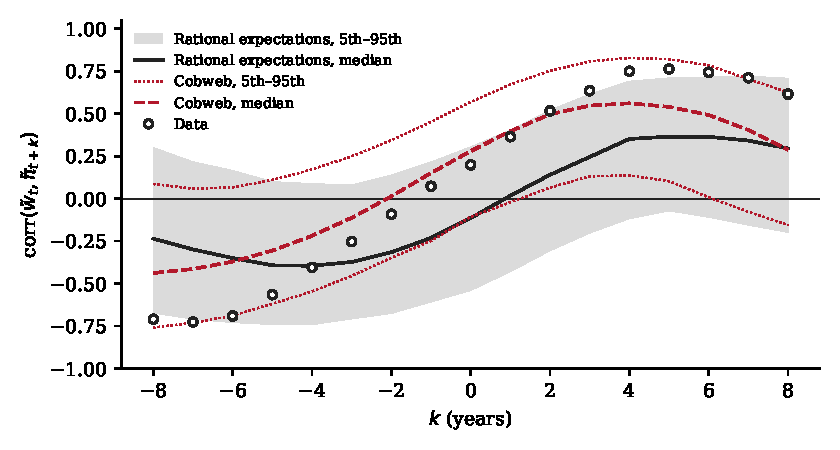
\includegraphics[width=0.64\linewidth]{fig_cw_leadcorr.pdf}
\caption{Correlation of the wage with the degree share $k$ years later}\label{fig:cwcorr}
\begin{minipage}{0.7\linewidth}\footnotesize
\textit{Notes:} Circles: data. Solid line and shaded band: median and 5th--95th percentile range across 1,000 simulated 43-year samples from the rational-expectations model. Dashed and dotted lines: the same for the cobweb model. Each sample is detrended as in the data.
\end{minipage}
\end{figure}

Figure \ref{fig:cwcorr} shows that the cobweb model matches the correlation between the wage and the future degree share. At $k=4$, its simulated median is 0.56 and its 5th--95th percentile range, $[0.14, 0.83]$, covers the value of 0.75 in the data. Students under the cobweb do not distinguish temporary from permanent wage changes: a 1 percent increase in the current wage raises enrollment by 5.1 percent on impact, against about 1.0 percent under rational expectations when the same increase comes from a demand shock. Enrollment follows the current wage closely, so the degree share four years later is strongly correlated with today's wage.

\begin{figure}[!htb]
\centering
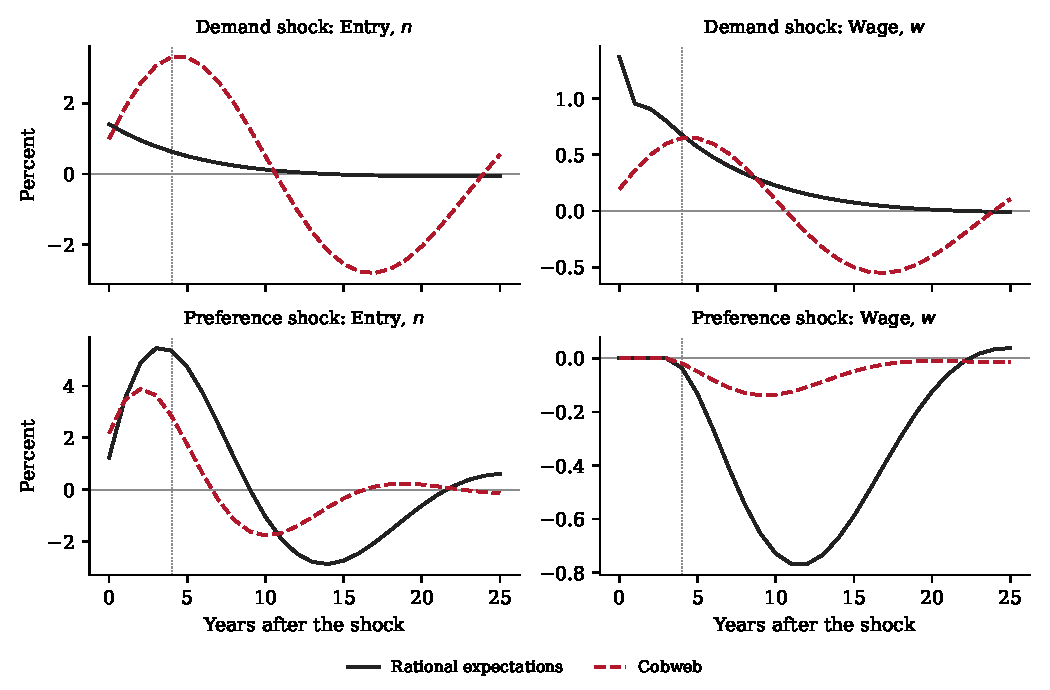
\includegraphics[width=0.62\linewidth]{fig_cw_irf.pdf}
\caption{Responses under rational expectations and the cobweb}\label{fig:cwirf}
\begin{minipage}{0.75\linewidth}\footnotesize
\textit{Notes:} Solid: rational expectations; dashed: cobweb. Each shock is one standard deviation as estimated in that model. The vertical dotted line marks year 4.
\end{minipage}
\end{figure}

Figure \ref{fig:cwirf} compares the impulse responses. Under a demand shock, the cobweb model produces the classic cobweb cycle: the wage rises, enrollment increases sharply, too many students graduate four years later, the wage falls back, and enrollment drops below normal. Part of this reversal, however, comes from the cycle in the demand shock itself. Under a preference shock, cobweb enrollment moves one for one with the shock for four years, because the wage has not yet changed, whereas under rational expectations enrollment rises on impact by only about 37 percent of the shock.

%%%%%%%%%%%%%%%%%%%%%%%%%%%%%%%%%%%%%%%%%%%%%%%%%%%%%%%%%%%%%%%%%%%%%%%%%%%%%%
\section{Conclusion}\label{sec:conclusion}

Estimating the Ryoo--Rosen model jointly by Kalman-filter maximum likelihood, we find that enrollment is highly sensitive to persistent wage changes under both rational and cobweb expectations, yet the large swings in the degree share come mainly from changes in the attractiveness of engineering, not from wages.

What the data cannot settle is whether students distinguish temporary from permanent wage changes. Since \citet{freeman1971market,freeman1976cobweb}, booms and busts in the market for engineers have often been explained as a cobweb cycle in which they do not, and our data do not reject this explanation; \citet[p.~S135]{ryoo2004engineering} similarly found it difficult ``to isolate the precise expectations mechanism.'' The cobweb model matches the link between wages and future degrees that the rational-expectations model misses, but only with a nearly flat demand curve and an almost deterministic long cycle in demand, and the two models' estimates of the demand elasticity differ by a factor of almost four.

Our numbers rest on several fixed choices: the discount factor is set at 0.96, each series is linearly detrended before estimation, the two shocks are independent, and enrollment involves no adjustment costs. The sample has only 43 annual observations, which bound the demand elasticity and the slope of the enrollment cost only from above, and about 81 percent of the variance of the observed stock is measurement error. These choices define the scope of our conclusions.

The framework itself is not specific to engineers. Occupations in which entry requires years of training and the return to entry depends on wages earned long afterward, such as physicians, lawyers, teachers, and scientists, share its structure. Given series on relative wages, stocks, and entry, the planning problem, the state-space representation, and the likelihood carry over, and estimates across occupations would show whether the patterns found here are particular to engineering.

\bibliographystyle{agsm}
\bibliography{references}

%%%%%%%%%%%%%%%%%%%%%%%%%%%%%%%%%%%%%%%%%%%%%%%%%%%%%%%%%%%%%%%%%%%%%%%%%%%%%%
\appendix

\section{Derivations for the Model}\label{app:derivations}

\subsection{Stock Accumulation}\label{app:stock}

Divide $L_{t+1} = \delta L_t + S_{t-3}$ by $L_t$. On a balanced growth path, $L_{t+1}/L_t = 1+g$ and $S_{t-3}/L_t = \bar{s}$, so $1+g = \delta + \bar{s}$. Let $\hat{\ell}_t$ and $\hat{s}_t$ be the log deviations of $L_t$ and $S_t$ from the path. A first-order expansion of $(1+g)e^{\hat{\ell}_{t+1} - \hat{\ell}_t} = \delta + \bar{s}\,e^{\hat{s}_{t-3} - \hat{\ell}_t}$ gives
\[
  (1+g)(\hat{\ell}_{t+1} - \hat{\ell}_t) = \bar{s}\,(\hat{s}_{t-3} - \hat{\ell}_t)
  \;\Longrightarrow\;
  \hat{\ell}_{t+1} = \lambda\,\hat{\ell}_t + (1-\lambda)\,\hat{s}_{t-3}, \qquad \lambda = \frac{\delta}{1+g} .
\]
With the same equation for all college graduates (superscript $c$), $N_t = \hat{\ell}_t - \hat{\ell}^{c}_t$, and $n_t = \hat{s}_t - \hat{s}^{c}_t$,
\[
  N_{t+1} = \lambda N_t + (1-\lambda)\, n_{t-3} + (\lambda - \lambda^{c})\big(\hat{\ell}^{c}_t - \hat{s}^{c}_{t-3}\big) .
\]
In our data the detrended standard deviation of the last term is 0.0022, against 0.0787 for $N_t$; dropping it gives \eqref{eq:stock}.

\subsection{The Household's Problem}\label{app:household}

Iterating the constraint in \eqref{eq:household}, $\partial N^{h}_{s}/\partial n_t = (1-\lambda)\lambda^{s-t-4}$ for $s \ge t+4$ and zero otherwise. Since the household takes wages as given, the derivative of its objective with respect to $n_t$, divided by $\beta^{t}$, is
\[
  -d\,(n_t - \psi_t) + (1-\lambda)\, E_t \sum_{j=0}^{\infty} \beta^{4+j} \lambda^{j}\, w_{t+4+j} = 0 ,
\]
which is \eqref{eq:hhfocmain}; the second derivative is $-d<0$. If $w_{t+k}$ rises by one unit for all $k \ge 0$, then $\Delta V_t = \beta^{4}\sum_{j\ge0}(\beta\lambda)^{j} = \beta^{4}/(1-\beta\lambda)$ and $\Delta n_t = \eta^{LR}$.

\subsection{Proof of Proposition \ref{prop:equivalence}}\label{app:equivalence}

Since $\partial(\theta_s N_s - \tfrac{f_2}{2}N_s^{2})/\partial N_s = \theta_s - f_2 N_s$, the planner's first-order condition for $n_t$ is
\begin{equation}\label{eq:plannerfoc}
  d\,(n_t - \psi_t) = (1-\lambda)\, E_t \sum_{j=0}^{\infty} \beta^{4+j}\lambda^{j}\,\big(\theta_{t+4+j} - f_2 N_{t+4+j}\big) .
\end{equation}
For $f_2, d > 0$ the objective is strictly concave and the constraints are linear, and for processes with bounded second moments $\beta < 1$ ensures the transversality condition. Hence $\{N_t, n_t\}$ solves \eqref{eq:planner} if and only if \eqref{eq:plannerfoc} holds for all $t$, and the solution is unique.

\textit{Necessity.} In an equilibrium, substituting the firm's condition $w_s = \theta_s - f_2 N_s$ into the household's condition \eqref{eq:hhfocmain} gives \eqref{eq:plannerfoc}.

\textit{Sufficiency.} Let $\{N_t, n_t\}$ satisfy \eqref{eq:plannerfoc} and set $w_s = \theta_s - f_2 N_s$, $N^{d}_s = N^{h}_s = N_s$. Then \eqref{eq:demand} and market clearing hold by construction, and \eqref{eq:plannerfoc} becomes \eqref{eq:hhfocmain}. Both private problems are strictly concave, so these first-order conditions are sufficient, and the allocation with this wage is an equilibrium. Uniqueness follows from that of the planner's solution. \hfill$\square$

\subsection{Linear-Quadratic Representation}\label{app:lq}

With $X_t$ and $u_t$ as in Section \ref{sec:planner}, the matrices in \eqref{eq:transition} are
{\small
\[
A = \begin{pmatrix}
\lambda & 0 & 0 & 1-\lambda & 0 & 0 & 0 & 0 & 0\\
0 & 0 & 0 & 0 & 0 & 0 & 0 & 0 & 0\\
0 & 1 & 0 & 0 & 0 & 0 & 0 & 0 & 0\\
0 & 0 & 1 & 0 & 0 & 0 & 0 & 0 & 0\\
0 & 0 & 0 & 1 & 0 & 0 & 0 & 0 & 0\\
0 & 0 & 0 & 0 & 0 & a^{\theta}_1 & 0 & a^{\theta}_2 & 0\\
0 & 0 & 0 & 0 & 0 & 0 & a^{\psi}_1 & 0 & a^{\psi}_2\\
0 & 0 & 0 & 0 & 0 & 1 & 0 & 0 & 0\\
0 & 0 & 0 & 0 & 0 & 0 & 1 & 0 & 0
\end{pmatrix},
\quad
B = \begin{pmatrix} 0\\1\\0\\0\\0\\0\\0\\0\\0 \end{pmatrix},
\quad
C = \begin{pmatrix} 0&0\\0&0\\0&0\\0&0\\0&0\\ \sigma_\theta&0\\ 0&\sigma_\psi\\ 0&0\\ 0&0 \end{pmatrix}.
\]
}
The only nonzero elements of $R$ are $R_{11} = -f_2/2$ and $R_{16} = R_{61} = 1/2$; $Q = -d/2$; and $W$ has $d/2$ in the position of $\psi_t$ and zeros elsewhere. These reproduce the period return in \eqref{eq:planner}.

\section{The Kalman Filter and the Likelihood}\label{app:kalman}

\subsection{The State-Space System}\label{app:ssm}

With $s_t = (X_t', v_t')'$ and $\epsilon_t = (\varepsilon^{\theta}_t, \varepsilon^{\psi}_t, e^{w}_t, e^{N}_t, e^{\pi}_t)' \sim \text{i.i.d. } N(0, I_5)$, the matrices in \eqref{eq:ssm} are
\[
  \mathcal{M} = \begin{pmatrix} M & 0 \\ 0 & D \end{pmatrix}, \qquad
  \mathcal{C} = \begin{pmatrix} C & 0 \\ 0 & \Sigma_v \end{pmatrix}, \qquad
  \mathcal{G} = \begin{pmatrix} G & I_3 \end{pmatrix},
\]
where $D = \mathrm{diag}(D_w, D_N, 0)$, $\Sigma_v = \mathrm{diag}(\sigma_w, \sigma_N, \sigma_\pi)$, and the rows of $G$ select $w_t = -f_2 N_t + \theta_t$, $N_t$, and $\pi_t = n_{t-4}$.

\subsection{The Filtering Recursions}\label{app:recursion}

Let $\Sigma_t = \mathrm{Var}(s_t \mid y^{t-1})$. Suppose $s_t \mid y^{t-1} \sim N(\hat{s}_t, \Sigma_t)$, which holds at $t=1$ with $\hat{s}_1 = 0$ and $\Sigma_1$ the stationary variance, $\Sigma_1 = \mathcal{M}\Sigma_1\mathcal{M}' + \mathcal{C}\mathcal{C}'$. Then $y_t \mid y^{t-1} \sim N(\mathcal{G}\hat{s}_t, \Omega_t)$ with $\Omega_t = \mathcal{G}\Sigma_t\mathcal{G}'$, and, conditional on $y^{t-1}$,
\[
  E[s_{t+1}] = \mathcal{M}\hat{s}_t, \qquad
  \mathrm{Var}(s_{t+1}) = \mathcal{M}\Sigma_t\mathcal{M}' + \mathcal{C}\mathcal{C}', \qquad
  \mathrm{Cov}(s_{t+1}, y_t) = \mathcal{M}\Sigma_t\mathcal{G}' .
\]
Conditioning further on $y_t$ with the formulas for jointly normal vectors gives
\begin{align*}
  \hat{s}_{t+1} &= \mathcal{M}\hat{s}_t + K_t a_t, \qquad K_t = \mathcal{M}\Sigma_t\mathcal{G}'\,\Omega_t^{-1}, \qquad a_t = y_t - \mathcal{G}\hat{s}_t, \\
  \Sigma_{t+1} &= \mathcal{M}\Sigma_t\mathcal{M}' + \mathcal{C}\mathcal{C}' - K_t\Omega_t K_t'
               = (\mathcal{M} - K_t\mathcal{G})\,\Sigma_t\,(\mathcal{M} - K_t\mathcal{G})' + \mathcal{C}\mathcal{C}' ,
\end{align*}
which completes the induction and yields \eqref{eq:innovrep}. The last form, a sum of positive semidefinite matrices, is the one used in Algorithm \ref{alg:loglik}.

\subsection{The Prediction Error Decomposition}\label{app:ped}

For $r < t$, $a_r$ is a function of $y^{t-1}$ and $E[a_t \mid y^{t-1}] = 0$, so $E[a_t a_r'] = 0$; being normal, the innovations are independent. The map from $y^{T}$ to $a^{T}$ is triangular with unit Jacobian. Hence
\[
  f(y_1, \dots, y_T) = \prod_{t=1}^{T} f\big(y_t \mid y^{t-1}\big)
  = \prod_{t=1}^{T} (2\pi)^{-3/2} \det(\Omega_t)^{-1/2} \exp\!\Big(-\tfrac12\, a_t'\Omega_t^{-1}a_t\Big) ,
\]
and taking logs gives \eqref{eq:loglik}, the exact Gaussian likelihood of the sample.

\section{Population Moments and Variance Decomposition}\label{app:moments}

The stationary variance of the state solves $\Sigma = \mathcal{M}\Sigma\mathcal{M}' + \mathcal{C}\mathcal{C}'$. Since $s_{t+k} = \mathcal{M}^{k}s_t$ plus innovations independent of $s_t$, the autocovariances of the observations are $\Gamma_k \equiv \mathrm{Cov}(y_{t+k}, y_t) = \mathcal{G}\mathcal{M}^{k}\Sigma\mathcal{G}'$, from which the population moments in Table \ref{tab:fit} follow. Let $\mathcal{C}_j$ be the $j$th column of $\mathcal{C}$. Because the components of $\epsilon_t$ are independent, $\mathcal{C}\mathcal{C}' = \sum_j \mathcal{C}_j\mathcal{C}_j'$, and by linearity of the Lyapunov equation $\Sigma = \sum_j \Sigma^{(j)}$ with $\Sigma^{(j)} = \mathcal{M}\Sigma^{(j)}\mathcal{M}' + \mathcal{C}_j\mathcal{C}_j'$. The share of shock $j$ in the variance of series $i$ is $[\mathcal{G}\Sigma^{(j)}\mathcal{G}']_{ii}/[\mathcal{G}\Sigma\mathcal{G}']_{ii}$; for the model variables in Table \ref{tab:vardecomp}, the same computation uses $M$, $C$, and the two structural shocks only.

\end{document}
